\documentclass[10pt]{article}
\usepackage[T1]{fontenc}
\usepackage{amsmath,amsfonts,amssymb}
\usepackage{mathtools}
\usepackage{color,soul}
\usepackage{fullpage}
\usepackage{enumerate}
\usepackage{graphicx}
\usepackage[colorlinks=true,urlcolor=blue]{hyperref}
\usepackage{subcaption}

\definecolor{Light}{gray}{.90}
\sethlcolor{Light}

\title{Skimmed 2D Images}
\author{Jeren Suzuki}
\date{Last Edited \today}

\begin{document}

\maketitle

\begin{figure}[!ht]
    \centering
    \includegraphics[width=.9\textwidth]{plots_tables_images/skimmilk.jpg}    
\end{figure}

\pagenumbering{Roman}
\tableofcontents
\newpage
\pagenumbering{arabic}

\section{Introduction} % (fold)
\label{sec:introduction}
An easier and faster way to crop our three suns in a single image is to find the brightest sun-like shape in our image, crop around it, set the area to zero, then find the next brightest sun-like shape. If we use sort to get a ``master array'' of positions and values, we can zero-out the parts of the image that are sun-like on the same array multiple times. The result is a fast and efficient cropping method.

% section introduction (end)

\section{1D Plot of a 2D image} % (fold)
\label{sec:1d_plot_of_a_2d_image}
We plot a 2D image as a 1D spectrum to identify the shapes in our 2D image.


\begin{figure}[!ht]
    \centering
    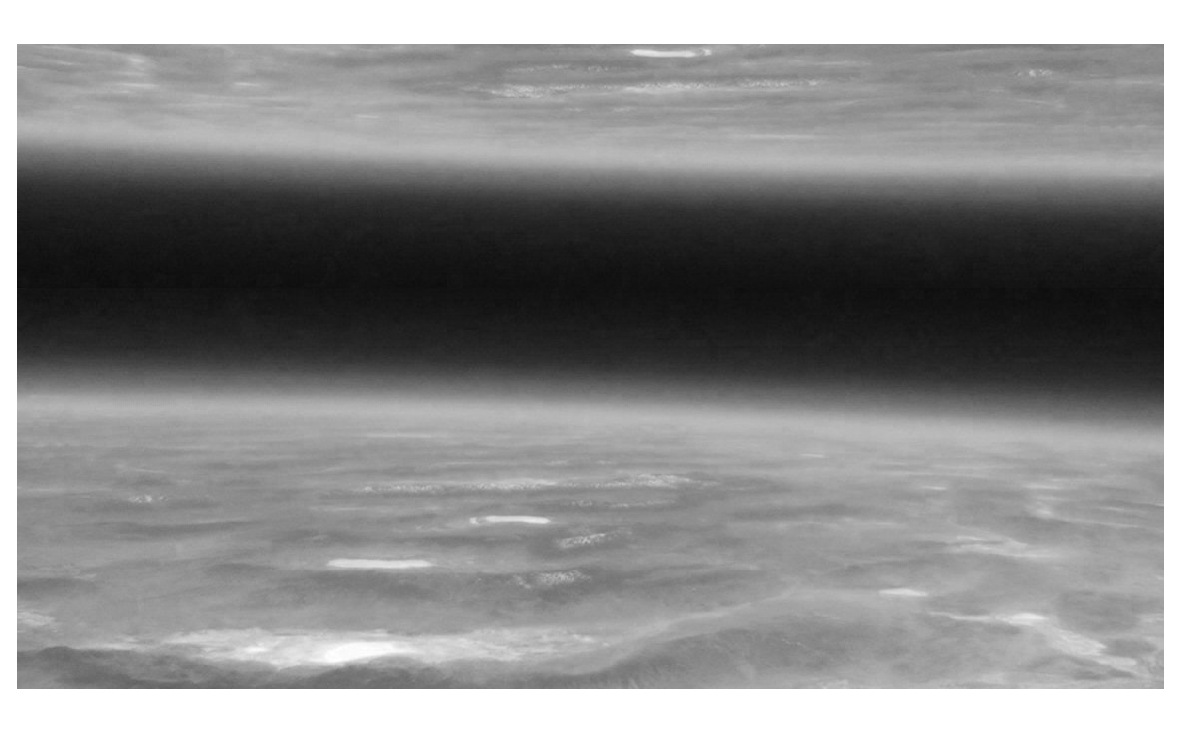
\includegraphics[width=.9\textwidth]{plots_tables_images/raw.eps}
    \caption{The raw 2D image we started out with. There are 7 pixels in this image equal to 255, the max brightness for a byte array. These pixels simulate abnormally high values in our image as a result of bad pixels, gamma rays, etc.}
    \label{raw}
\end{figure}

Starting from Figure \ref{raw}, we plotted the lowest 99\% of the pixels when ordered by brightness to eliminate the abnormally high pixels to get Figure \ref{sorted}.

\begin{figure}[!ht]
    \centering
    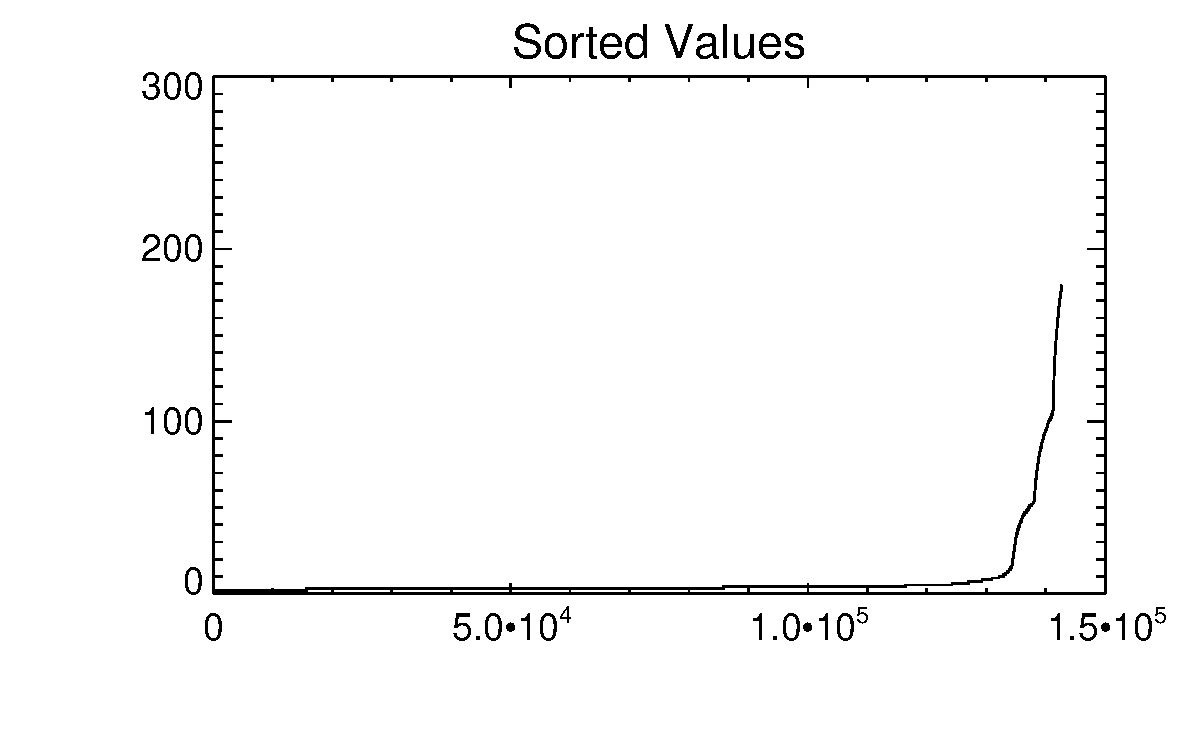
\includegraphics[width=.9\textwidth]{plots_tables_images/sorted_array.eps}
    \caption{Lowest 99\% of sorted 2D image.}
    \label{sorted}
\end{figure}

We see three distinct humps, indicative of our three suns in the 2D image. Now, to find the boundaries where one sun ends and the other begins, we look at the derivative of Figure \ref{sorted}. However, simply taking the derivative does not result in a usable result so we must smooth our data first. I use both \texttt{\hl{smooth()}} and \texttt{\hl{ts\_smooth()}} in Figure \ref{comps}.

\begin{figure}[!ht]
    \centering 
    \hspace{-1.0in}
    \begin{subfigure}[b]{.45\linewidth}
        \centering
        \includegraphics[width=1.3\textwidth]{plots_tables_images/d_ts.eps}
    \end{subfigure}
    \hspace{.5in}
    \begin{subfigure}[b]{.45\linewidth}
        \centering
        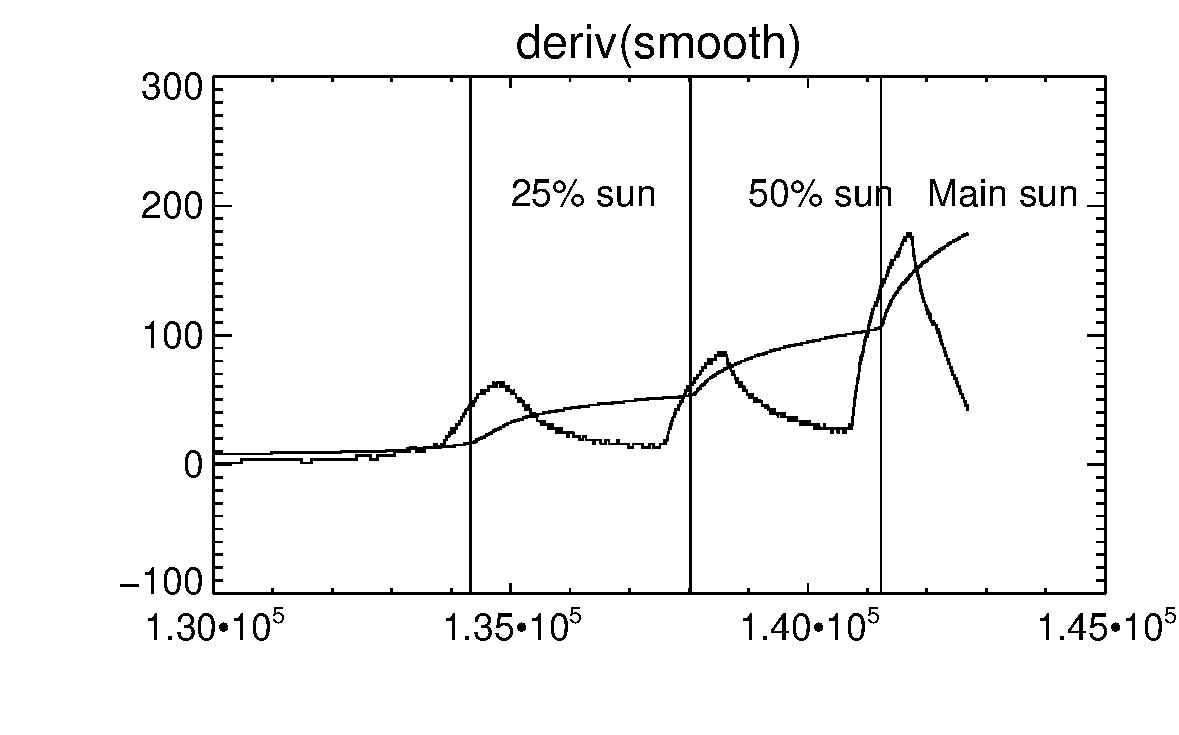
\includegraphics[width=1.3\textwidth]{plots_tables_images/d_reg.eps}
    \end{subfigure}
   
   \hspace{-1.0in}
   \begin{subfigure}[b]{.45\linewidth}
        \centering
        \includegraphics[width=1.3\textwidth]{plots_tables_images/d_ts_d_ts.eps}
    \end{subfigure}
    \hspace{.5in}
    \begin{subfigure}[b]{.45\linewidth}
        \centering
        \includegraphics[width=1.3\textwidth]{plots_tables_images/d_ts_d_reg.eps}
    \end{subfigure}

    \hspace{-1.0in}
    \begin{subfigure}[b]{.45\linewidth}
        \centering
        \includegraphics[width=1.3\textwidth]{plots_tables_images/d_s_d_ts.eps}
    \end{subfigure}
    \hspace{.5in}
    \begin{subfigure}[b]{.45\linewidth}
        \centering
        \includegraphics[width=1.3\textwidth]{plots_tables_images/d_s_d_reg.eps}
    \end{subfigure}
    \caption{The vertical lines correspond to eyeballed boundaries of the sorted array. A large part of the left half of the array is cropped out to emphasize the shape of the humps and peaks. The derivative has been scaled to within the max/min of the starting master array.}
    \label{comps}
\end{figure}

It turns out that \texttt{\hl{ts\_smooth}} takes an incredibly long time to run when the order of the autoregressive model is greater than 10. As such, I chose an order of 3 so that it didn't take too long. Even then, running a simple \hl{\texttt{smooth()}} filter results in some pretty good plots. It's important to note that the derivative must be smoothed before I can take another another derivative; also, it doesn't seem to matter if I use \texttt{\hl{ts\_smooth}} or \hl{\texttt{smooth()}} when taking the second smooth.

% section 1d_plot_of_a_2d_image (end)


\section{Drawbacks} % (fold)
\label{sec:drawbacks}
    The biggest problem with this method is that the pixel values overlap somewhat with different regions. Say the brightest region, region 1, is in the center of our image. Region 2 is at a brightness 50\% of the main sun. Say we now arrange the 2D plot as a 1D array and see two bumps, one for each solar region. Now, region 2 is intrinsically dimmer than region 1, which means there are going to be pixels in region 2 that will be comparative to the dark limb pixels of region 1. Since our 1D array (now that it's sorted, especially) has no spatial information, we cannot tell two pixels apart that have the same value but are in different regions. 
% section drawbacks (end)

\end{document}










